\section{Vorbereitung}

Die Vorbereitungsphase umfasst die Umstellung auf FreeRTOS und damit die
vollständige Ablösung von Micro-ROS. Der Datenaustausch wird intern über
FreeRTOS-Queues realisiert, während die Task-Synchronisation auf
Direct-Task-Notification anstatt von Semaphoren basiert. Zusätzlich wird die
Eingabe von Sollgeschwindigkeiten über UART mit CRC implementiert. Die
Aktivierung des Caches bildet den Abschluss dieser Vorbereitungen. Die Details
zu diesen Maßnahmen werden in den folgenden Abschnitten erläutert.

\subsection{Umstellung auf FreeRTOS}

\subsubsection{Geschwindigkeitsempfang über UART auf Mikrocontroller}

In der bisherigen Implementierung wurde der Geschwindigkeitssollwert vom Host
über ROS2 von dem Micro-ROS-Agent an den Client auf den MCU übertragen. Um die
Abhängigkeit von Micro-ROS komplett zu beseitigen, muss die Übertragung und
Interpretierung der Geschwindigkeitssollwerte manuell implementiert werden.

Es wird zunächst ein einfacher Struct \mintinline{cpp}|Vel2d| definiert, um die
Geschwindigkeitswerte zu interpretieren, die vom Benutzer an den MCU gesendet
werden.

\begin{code}
\begin{minted}{cpp}
struct Vel2d {
  double x;
  double y;
  double z;
};
\end{minted}
    \captionof{listing}{Definition der Struktur für die Sollgeschwindigkeit}
\end{code}

Darauf aufbauend wird eine weitere Struct \mintinline{cpp}|Vel2dFrame|
definiert, die als UART-Daten-Frame dient. Dieser enthält ein zusätzliches Feld
\mintinline{cpp}|crc| für die CRC-Überprüfung und eine Methode
\mintinline{cpp}|compare()|, die einen lokal kalkulierten CRC-Wert als Parameter
entgegennimmt, um diesen mit dem empfangenen zu vergleichen. Mit dem Attribut
\linebreak\mintinline{cpp}|__attribute__((packed))| wird verhindert, dass
zusätzliches Padding für die Speicherausrichtung dieses Typs eingefügt wird,
Damit die über UART empfangenen Bytes direkt als Objekt dieses Typs
interpretiert werden können.

\begin{code}
\begin{minted}{cpp}
struct Vel2dFrame {
  Vel2d vel;
  uint32_t crc;

  bool compare(uint32_t rhs) { return crc == rhs; }
} __attribute__((packed));

inline constexpr std::size_t VEL2D_FRAME_LEN = sizeof(Vel2dFrame);
\end{minted}
    \captionof{listing}{Definition der Data-Frame für die Sollgeschwindigkeit}
\end{code}

Für die Übertragung über UART kann die Setup-Funktion \linebreak
\mintinline{cpp}|HAL_UARTEx_ReceiveToIdle_IT()| aus der STM32-HAL-Bibliothek
verwendet werden, um die serialisierten Bytes eines Data-Frames zu empfangen.
Sie nimmt das UART-Handle, die Adresse eines Datenpuffers und dessen Größe
entgegen und empfängt die eingehenden Daten über Interrupts in diesen vorab
zugewiesenen Puffer.

Dies ist gepaart mit einer Interrupt-Callback
\mintinline{cpp}|HAL_UARTEx_RxEventCallback()|, die entweder ausgelöst wird,
wenn - wie der Name der UART-Setup-Funktion bereits andeutet - die UART-Leitung
feststellt, dass die Übertragung für eine bestimmte Zeit (abhängig von der
Baudrate) inaktiv war, oder wenn der Puffer für die Übertragung voll ist, was
darauf hinweist, dass der gesamte Inhalt des Puffers verarbeitet werden kann
\cite{HAL_UARTEx_ReceiveToIdle_IT}. Der zweite Parameter dieser
Interrupt-Callback gibt die Größe der in den Puffer geschriebenen Daten an
\cite{HAL_UARTEx_RxEventCallback}.

Mit diesem Setup kann die Software nun Bytes beispielsweise über UART direkt von
einem Linux-Host-Rechner empfangen, der mit dem MCU-Board verbunden ist.

\begin{code}
\begin{minted}{cpp}
// preallocated buffer with the exact size of a data frame
static uint8_t uart_rx_buf[VEL2D_FRAME_LEN];
volatile static uint16_t rx_len;

void HAL_UARTEx_RxEventCallback(UART_HandleTypeDef* huart, uint16_t size) {
  if (huart->Instance != huart3.Instance) return;

  rx_len = size;
  static BaseType_t xHigherPriorityTaskWoken;
  configASSERT(task_handle != NULL);
  vTaskNotifyGiveFromISR(task_handle, &xHigherPriorityTaskWoken);
  portYIELD_FROM_ISR(xHigherPriorityTaskWoken);

  // reset reception from UART
  HAL_UARTEx_ReceiveToIdle_IT(&huart3, uart_rx_buf, sizeof(uart_rx_buf));
}

// setup reception from UART in task init
HAL_UARTEx_ReceiveToIdle_IT(&huart3, uart_rx_buf, sizeof(uart_rx_buf));
\end{minted}
    \captionof{listing}{Nutzung STM32-API für den Datenempfang über UART via
    Interrupt}
\end{code}

Um die empfangenen Bytes zu parsen, ohne dies aber während der Ausführung der
Interrupt-Callback zu tun, wird eine eigenständige FreeRTOS-Task erstellt.
Dieser Task wird von der Interrupt-Callback mittels
\mintinline{cpp}|vTaskNotifyGiveFromISR()|
signalisiert~\ref{sec:direct_task_notification} und die empfangenen Bytes werden
wieder in ein Data-Frame deserialisiert, um die Geschwindigkeit und die CRC zu
extrahieren.

Demnach kann dann eine CRC zur Kontrolle lokal aus den empfangenen
Geschwindigkeitswert berechnet werden und sie mit der empfangenen vergleichen.
Durch die Nutzung der dedizierten CRC-Peripherie ist die Berechnung
beispielsweise auf einem STM32-F37x-Gerät das 60-fache schneller, und verwendet
dabei nur 1,6\% der Taktzyklen im Vergleich zur Softwareberechnung \cite[S.
9]{AN4187}.

\begin{code}
\begin{minted}{cpp}
  while (true) {
    ulTaskNotifyTake(pdTRUE, portMAX_DELAY);

    len = rx_len;  // access atomic by default on ARM
    if (len != VEL2D_FRAME_LEN) {
      ULOG_ERROR("parsing velocity failed: insufficient bytes received");
      continue;
    }

    auto frame = *reinterpret_cast<const Vel2dFrame*>(uart_rx_buf);
    auto* vel_data = reinterpret_cast<uint8_t*>(&frame.vel);
    if (!frame.compare(HAL_CRC_Calculate(
            &hcrc, reinterpret_cast<uint32_t*>(vel_data), sizeof(frame.vel)))) {
      ULOG_ERROR("crc mismatch!");
      ++crc_err;
      continue;
    }

    frame.vel.x *= 1000;  // m to mm
    frame.vel.y *= 1000;  // m to mm

    xQueueSend(freertos::vel_sp_queue, &frame.vel, NO_BLOCK);
  }
\end{minted}
    \captionof{listing}{FreeRTOS-Task Dauerschleife}
\end{code}

\subsubsection{Geschwindigkeitsübertragung über UART auf Host}

Um den vom Benutzer festzulegenden Geschwindigkeitssollwert für den mobilen
Roboter zu übertragen, ist dem MCU-Board, auf dem die Steuerungssoftware läuft,
physisch per UART mit einem Linux-Host (einem Raspberry Pi 5) verbunden. Auf dem
Host wird das vorhandene ROS2-Paket \mintinline{text}|teleop_twist_keyboard|
weiter verwendet, um Geschwindigkeitseingaben des Benutzers über die Tastatur zu
interpretieren. Um die Werten dann über UART zu übertragen, wird ein kleiner
ROS2-Node als Brücke erstellt, der die Funktion des Micro-ROS-Agents ersetzt.

Dabei empfängt der Node über das ROS2-Framework die Geschwindigkeitssollwerte
und überträgt sie zusammen mit der im Konstruktur kalkulierten CRC an die
UART-Schnittstelle, die auf Linux als abstrahierter serieller Port geöffnet ist.

\begin{code}
\begin{minted}{cpp}
class Vel2dBridge : public rclcpp::Node {
 public:
  Vel2dBridge() : Node{"vel2d_bridge"} {
    twist_sub_ = create_subscription<Twist>(
        "cmd_vel", 10, [this](Twist::UniquePtr twist) {
          auto frame =
              Vel2dFrame{{twist->linear.x, twist->linear.y, twist->angular.z}};

          if (!uart.send(frame.data())) {
            RCLCPP_ERROR(this->get_logger(), "write failed");
            return;
          }
          RCLCPP_INFO(this->get_logger(), "sending [%f, %f, %f], crc: %u",
                      frame.vel.x, frame.vel.y, frame.vel.z, frame.crc);
        });
  }

 private:
  rclcpp::Subscription<Twist>::SharedPtr twist_sub_;
  SerialPort<VEL2D_FRAME_LEN> uart =
      SerialPort<VEL2D_FRAME_LEN>(DEFAULT_PORT, B115200);
};
\end{minted}
    \captionof{listing}{ROS2-Node Implementierung für
    Geschwindigkeitsübertragung}
\end{code}

Die CRC-Berechnung auf dem Host erfolgt mithilfe einer C++-Bibliothek von Daniel
Bahr \cite{CRCpp}. Der Algorithmus \mintinline{cpp}|CRC::CRC_32_MPEG2()|
entspricht demjenigen, der von der CRC-Peripherie des STM32-Boards verwendet
wird.

\begin{code}
\begin{minted}{cpp}
Vel2dFrame::Vel2dFrame(Vel2d vel)
    : vel{std::move(vel)},
      crc{CRC::Calculate(&vel, sizeof(vel), CRC::CRC_32_MPEG2())} {}
\end{minted}
    \captionof{listing}{CRC-Berechnung im Konstruktur}
\end{code}

Mithilfe dieser Implementierungen werden die Übertragung der
Geschwindigkeitssollwerte vom Host und deren Empfang auf dem MCU ermöglicht.
Dadurch, dass der Empfang detektiert, dass keine weiteren Bytes übertragen
werden, und ebenso durch die Überprüfung der CRC, werden unvollständige oder
fehlerhafte Bytes erkannt und verworfen, ohne den Programmablauf zu blockieren.

\subsubsection{Steuerungskomponenten als FreeRTOS-Tasks}

Analog zur Implementierung basierend auf Micro-ROS, bei der alle logischen
Komponenten als Single-Threaded-Executor abstrahiert werden, sind diese
Komponenten in FreeRTOS ebenfalls als eigenständige Tasks implementiert. Der
Fokus liegt hierbei darauf, den grundlegenden Datenaustausch in Form einer
Publisher-Subscriber-Architektur mittels Queues zu realisieren. Dadurch müssen
die Daten nicht mehr durch Semaphoren oder Mutexe geschützt werden, welche in
FreeRTOS auch nur mittels Queue-Objekte abstrahiert sind.

Zunächst wird eine eigenständige Task zur Abfrage und Übertragung der
Encoderwerte erstellt, die von der Hardware bzw. der Hardwareabstraktion durch
Timer bereitgestellt werden, damit die anderen Tasks bei jeder Iteration auf
einheitliche Encoderwerte zugreifen können.

\begin{code}
\begin{minted}{cpp}
static void task_impl(void*) {
  constexpr TickType_t NO_BLOCK = 0;
  TickType_t xLastWakeTime = xTaskGetTickCount();
  const TickType_t xFrequency = pdMS_TO_TICKS(WHEEL_CTRL_PERIOD_MS.count());

  while (true) {
    auto enc_delta = FourWheelData(hal_encoder_delta_rad());

    xQueueSend(freertos::enc_delta_wheel_ctrl_queue, &enc_delta, NO_BLOCK);
    xQueueOverwrite(freertos::enc_delta_odom_queue, &enc_delta);

    vTaskDelayUntil(&xLastWakeTime, xFrequency);
  }
}
\end{minted}
    \captionof{listing}{FreeRTOS-Task für Encoderwertabfrage und -übertragung}
\end{code}


Die Empfänger-Task, welche mit \mintinline{cpp}|xQueueSend()| addressiert wird,
läuft mit einer höhreren Frequenz, sodass er die Daten immer schneller
verarbeitet und auf neue Daten wartet. Im Gegensatz dazu ist
\mintinline{cpp}|xQueueOverwrite()| eine spezielle Funktion, die ausschließlich
für Queues mit einer maximalen Kapazität von einem Objekt vorgesehen ist. Sie
überschreibt das vorhandene Objekt in der Queue, falls es existiert. In diesem
Kontext ist dies jedoch irrelevant, da die zugehörige Empfänger-Task, der mit
der gleichen Frequenz wie die Encoderwert-Task läuft, die Daten synchron
verarbeitet. Dennoch dient die Überschreibbarkeit als zusätzliche
Sicherheitsmaßnahme für den Fall einer Verzögerung.

Darauf basierend kann die Kommunikation als Matrix wie folgt illustriert werden:

\begin{table}[h!]
\centering
\small
\setlength{\tabcolsep}{4pt} % Reduce column padding
\begin{tabular}{|c|c|c|c|}
\hline
    \diagbox{Sendertask}{Empfängertask} & \textbf{Odometrie} & \textbf{Drehzahlregelung} & \textbf{Posenregelung} \\ \hline
\textbf{Encoderwerte}               & $\rightarrow$             & $\rightarrow$       &               \\ \hline
\textbf{Geschwindigkeitssollwert}   &                           &                     & $\rightarrow$ \\ \hline
\textbf{Odometrie}                  & \cellcolor{gray!20}       &                     & $\rightarrow$ \\ \hline
\textbf{Drehzahlregelung}           &                           & \cellcolor{gray!20} & $\rightarrow$ \\ \hline
\end{tabular}
\caption{Kommunikationskanal-Matrix}
% \label{tab:kommunikationsmatrix}
\end{table}

Die Kanäle werden dementsprechend durch Queue-Objekte repräsentiert.

\begin{code}
\begin{minted}{cpp}
extern QueueHandle_t enc_delta_odom_queue;
extern QueueHandle_t enc_delta_wheel_ctrl_queue;
extern QueueHandle_t vel_sp_queue;
extern QueueHandle_t odom_queue;
extern QueueHandle_t vel_wheel_queue;
\end{minted}
    \captionof{listing}{Queue-Objekte in FreeRTOS}
\end{code}

Die grundlegende Implementierung der jeweiligen Steuerungstasks bleibt
größententeils von der Micro-ROS-Struktur erhalten. Die Initialisierung der
jeweiligen Steuerungstasks erfolgt in \mintinline{cpp}|freertos::init()|:

\begin{code}
\begin{minted}{cpp}
void init() {
  hal_init();
  queues_init();
  task_hal_fetch_init();
  task_vel_recv_init();
  task_pose_ctrl_init();
  task_wheel_ctrl_init();
  task_odom_init();
}
\end{minted}
    \captionof{listing}{Initialisierung von FreeRTOS-Tasks}
\end{code}

Eine üblicher Ansatz in einem FreeRTOS-System, um unter anderem sowohl den
Speicherverbrauch zu optimieren als auch die Programmdeterminiertheit zu
verbessern, besteht darin, die Erstellung der FreeRTOS-Objekte statisch
durchzuführen \cite{freertos_memory_management}.

Um diese zu realisieren, wird im Makefile ein Macro
\mintinline{text}|-DFREERTOS_STATIC_INIT| definiert, das zur
Übersetzungszeit festlegt, ob die Objekte dynamisch innerhalb der FreeRTOS-API
oder statisch mit benutzerdefinierten Speicherorten zugewiesen werden sollen.

Für eine Task, der dynamisch allokiert wird, ist der Funktionsaufruf so einfach
wie der folgende:

\begin{code}
\begin{minted}{cpp}
xTaskCreate(task_impl, "hal_fetch", STACK_SIZE,
            NULL, osPriorityNormal, &task_handle);
\end{minted}
    \captionof{listing}{Dymanische Allokation eines FreeRTOS-Tasks}
\end{code}

Wenn eine Task statisch allokiert werden soll, muss der Benutzer manuell jeweils
einen Speicherpuffer für den Task-Stack und für die Task selbst deklarieren und
an die API übergeben.

\begin{code}
\begin{minted}{cpp}
static StackType_t taskStack[STACK_SIZE];
static StaticTask_t taskBuffer;
task_handle = xTaskCreateStatic(
                    task_impl, "hal_fetch", STACK_SIZE, NULL, osPriorityNormal,
                    taskStack, &taskBuffer);
\end{minted}
    \captionof{listing}{Dymanische Allokation eines FreeRTOS-Tasks}
\end{code}

Analog dazu muss der Benutzer für die statische Allokation einer Queue auch
jeweils einen Speicherpuffer mit der maximalen Kapazität für die Queue und die
Queue-Struktur selbst deklarieren:

\begin{code}
\begin{minted}{cpp}
 constexpr size_t QUEUE_SIZE = 10;
 static FourWheelData buf[QUEUE_SIZE];
 static StaticQueue_t static_queue;
 return xQueueCreateStatic(QUEUE_SIZE, sizeof(*buf),
                           reinterpret_cast<uint8_t*>(buf), &static_queue);
\end{minted}
    \captionof{listing}{Dymanische Allokation einer FreeRTOS-Queue}
\end{code}

Damit schließt der Abschnitt zur Umstellung auf FreeRTOS. Der Code für die
MCU-Software sowie für den ROS2-Node auf dem Host ist im
Repository~\cite{mecarover_freertos_profiling} verfügbar.

\subsection{Aktivierung von Instruktionscache}

Zum Aktivieren des Instruktionscaches muss die Funktion
\mintinline{cpp}|SCB_EnableICache()| aufgerufen werden. Da der Instruktionscache
ausschließlich schreibgeschützte Befehle zwischenspeichert, ist keine
Synchronisation mit modifizierbaren Daten erforderlich.

\subsection{Aktivierung von Datencache}

Obwohl der Datencache durch den einfachen Funktionsaufruf
\mintinline{cpp}|SCB_EnableDCache()| aktiviert wird, stellt dies jedoch noch
nicht den abschließenden Schritt dar.

Die Transportfunktionen für Micro-ROS nutzen die Ethernet-Schnittstelle, deren
Funktionalität durch die Integration des LwIP-Stacks, der intern DMA verwendet,
erweitert wird. Um sicherzustellen, dass die Daten korrekt verarbeitet werden,
müssen sowohl der Heap für LwIP als auch die Speicherbereiche für die
Ethernet-RX- und TX-Deskriptoren mittels \ac{MPU} so konfiguriert werden, dass
sie nicht gecacht werden \cite{STM32H7_LwIP_Examples}.

\begin{figure}[htb]
    \centering
    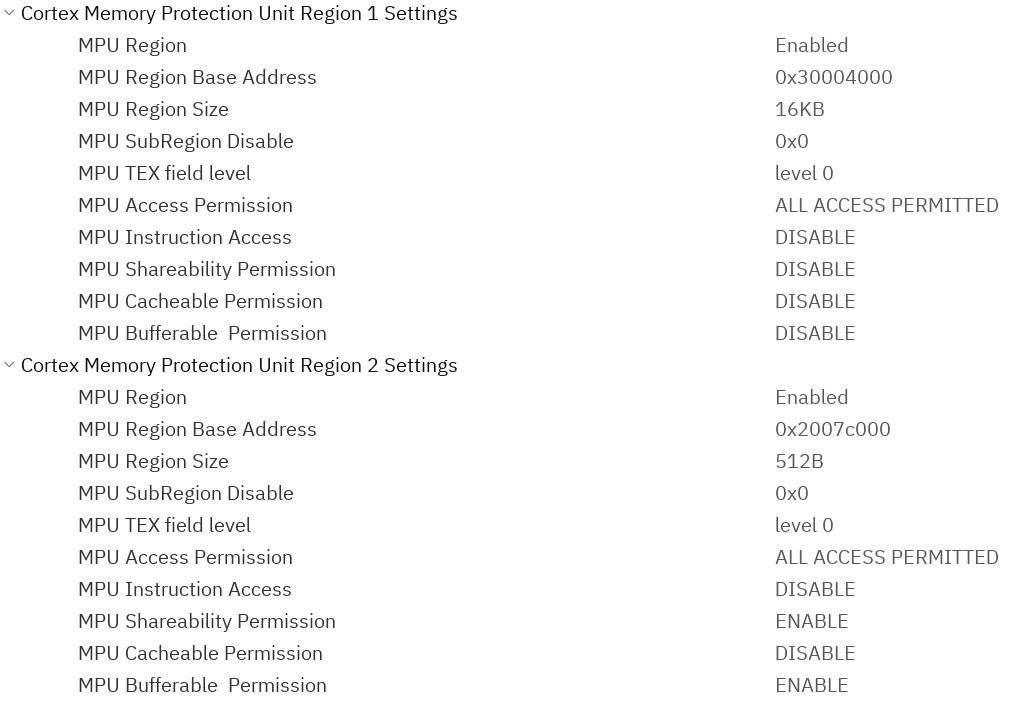
\includegraphics[width=1\textwidth]{assets/mpu_conf_cubemx}
    \caption{MPU-Konfiguration aus STM32CubeMX}
\end{figure}

Hierbei werden die Anfangsadressen sowie die Größe der RX- und TX-Deskriptoren
und des LwIP-Heaps aus CubeMX entnommen. Wichtig ist es, die Zugriffsrechte
(Access Permission) korrekt zu konfigurieren und sicherzustellen, dass der Cache
(Cacheable Permission) deaktiviert ist.

Obwohl die MPU konfiguriert wurde, um die Speicherbereiche für LwIP und die
Ethernet-Deskriptoren als nicht-cachebar zu markieren, tritt dennoch ein Fehler
auf, sobald die Verbindung zum Micro-ROS-Agent auf dem Host hergestellt wird.
Der Fehler (\ref{fig:micro_ros_err}), der in den Debugausgaben des
Micro-ROS-Agents sichtbar ist, deutet darauf hin, dass auf der Low-Level-Ebene
bei der Übertragung der Daten über UDP weiterhin Probleme mit der Cache-Kohärenz
auftreten. Insbesondere scheint das \mintinline{text}|client_key| oder die
assoziierten Daten nicht korrekt gecacht zu werden.

\begin{figure}[htb]
    \centering
    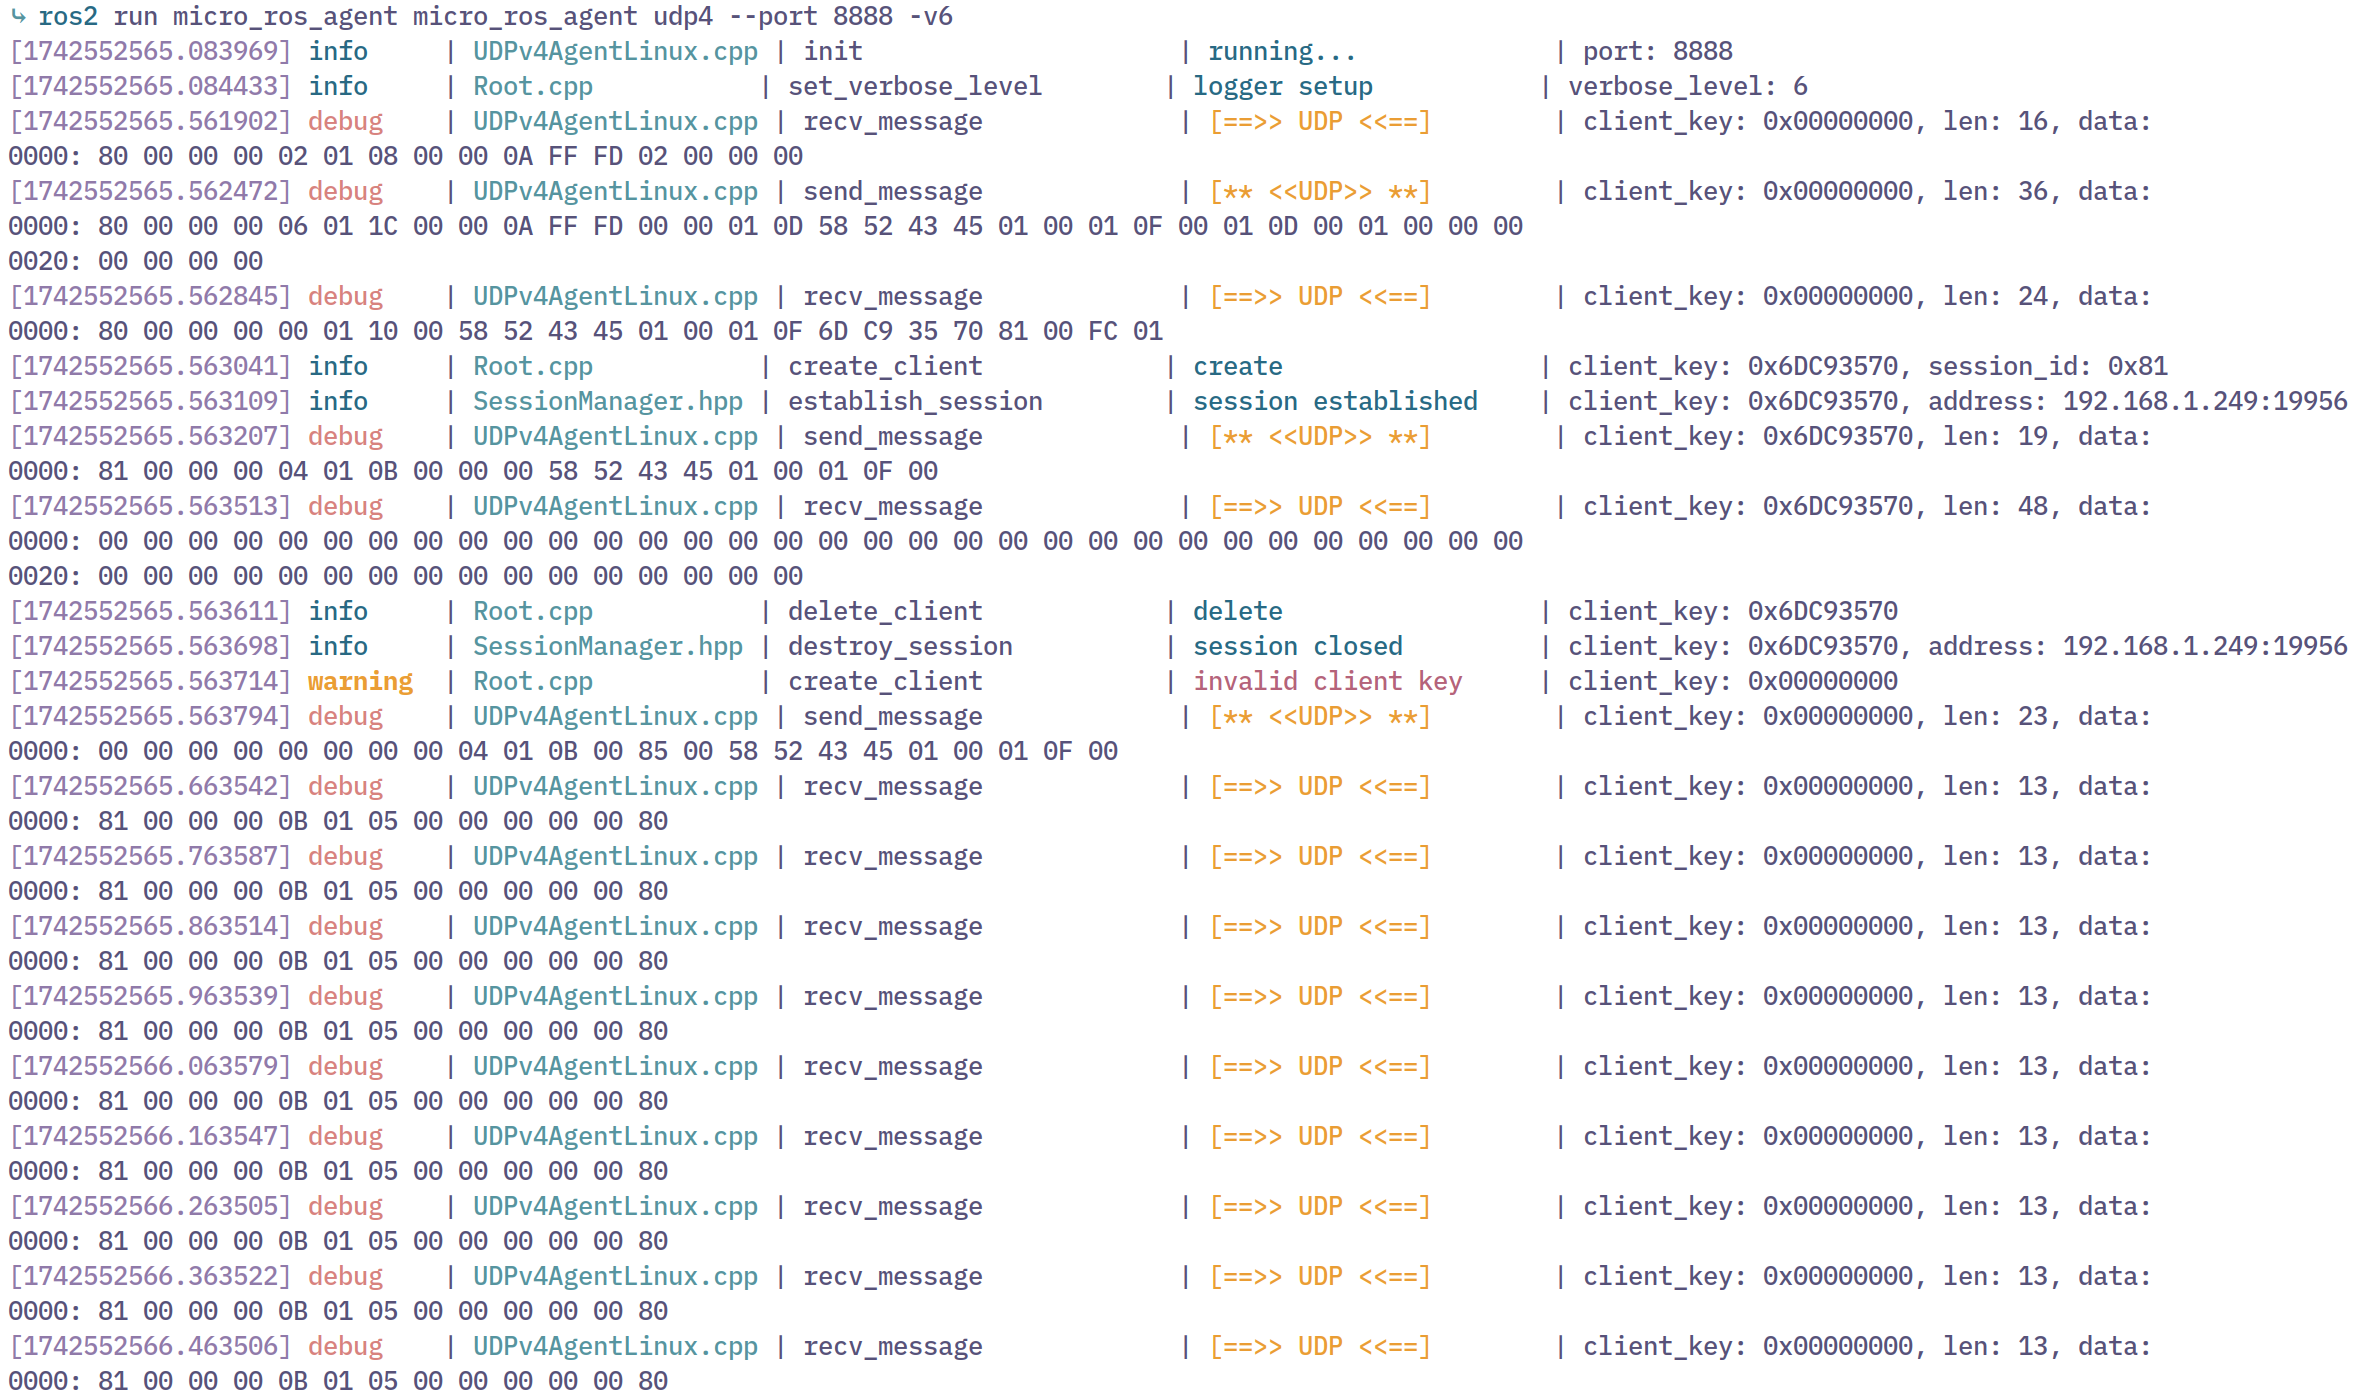
\includegraphics[width=1\textwidth]{assets/micro_ros_agent_err}
    \caption{Micro-ROS-Agent Fehlermeldung mit Debugausgaben}
    \label{fig:micro_ros_err}
\end{figure}

Bei der Recherche zu diesem Problem wurde ein Issue auf GitHub identifiziert,
welches genau das selbe Verhalten beschrieb. In diesem Kontext wurde dann der
Autor um eine Lösung gebeten, die daraufhin bereitgestellt wurde und sich als
effektiv erwies, um das Problem zu beheben \cite{microROS_STM32CubeMX_Issue139}.

\begin{code}
\begin{minted}{diff}
@@ -54,6 +54,10 @@
 /* USER CODE BEGIN 1 */
 /* address has to be aligned to 32 bytes */
+#define ALIGN_ADDR(addr) ((uintptr_t)(addr) & ~0x1F)
+#define ALIGN_SIZE(addr, size) ((size) + ((uintptr_t)(addr) & 0x1f))
+#define FLUSH_CACHE_BY_ADDR(addr, size) \
+  SCB_CleanDCache_by_Addr((uint32_t *)ALIGN_ADDR(addr), ALIGN_SIZE(addr, size))
 /* USER CODE END 1 */
 
 /* Private variables ---------------------------------------------------------*/
@@ -404,6 +408,8 @@
     Txbuffer[i].buffer = q->payload;
     Txbuffer[i].len = q->len;
 
+    FLUSH_CACHE_BY_ADDR(Txbuffer[i].buffer, Txbuffer[i].len);
+
     if(i>0)
     {
       Txbuffer[i-1].next = &Txbuffer[i];
\end{minted}
    \captionof{listing}{Modifizierung des ST-Treiber-Quellcode in Diffansicht}
\end{code}

Die Lösung ist in Bezug auf den Codeumfang recht simple: Für jede Übertragung
muss nur der Cache für die Payload jedes Paketpuffers (\mintinline{cpp}|pbuf|)
in \mintinline{cpp}|low_level_output()| mittels den Funktionsaufruf
\mintinline{cpp}|SCB_CleanDCache_by_Addr()| geleert werden, um einen sogenannten
Cache-Writeback auszulösen (\ref{sec:cache_clean}), so dass die Änderungen
tatsächlich in den Speicher geschrieben und somit auch beim DMA-Controller
korrekt widergespiegelt werden. Diese Lösung ist ebenfalls in einem Beitrag aus
dem Jahr 2018 im ST-Forum dokumentiert \cite{ST_Forum_Post_2018}.

Da die Größe jeder Cacheline auf allen Cortex-M7-Prozessoren 32 Byte beträgt
~\cite[S. 4]{an4839} und bei jedem Caching die gesamte Cacheline gefüllt wird,
selbst wenn die Daten weniger als 32 Byte umfassen, muss die angegebene Adresse
der Daten, deren Cache geleert werden soll, durch eine bitweise AND-Operation
mit \mintinline{text}|~0x1F| auf eine 32-Byte-Grenze ausgerichtet
werden~\cite{CMSIS_Core_CacheFunctions}. Nach der Anpassung der Adresse für die
32-Byte-Ausrichtung muss auch die Größe entsprechend ergänzt werden, um die
fehlenden Bytes nach der Ausrichtung zu berücksichtigen.

Hierbei ist zu beachten, dass ein Teil der Modifizierung direkt im generierten
ST-Treiber-Quellcode vorgenommen wird, der bei jeder Neugenerierung
überschrieben wird. In der Funktion \mintinline{cpp}|low_level_output()| ist
kein durch ST bereitgestellter User-Code-Guard vorhanden, und ein manuell
hinzugefügter User-Code-Guard wird ebenfalls überschrieben. Um dieses Problem zu
umgehen, wurde eine Patch-Datei erstellt, die nach jeder Generierung der
Konfigurationsdateien auf die Quelldatei \linebreak
\mintinline{text}|LWIP/Target/ethernetif.c| angewendet werden muss.
